\documentclass[11pt,a4paper]{article}

\usepackage{amsmath,amssymb,amsthm,mathtools}
\usepackage{booktabs,array,enumitem}
\usepackage{tikz}
\usetikzlibrary{positioning,arrows.meta,calc}
\usepackage[margin=2.5cm]{geometry}
\usepackage{microtype}
\usepackage[colorlinks=true,linkcolor=blue!50!black,citecolor=blue!50!black,urlcolor=blue!50!black]{hyperref}

% ---------- theorem-like environments ----------
\theoremstyle{definition}
\newtheorem{definition}{Definition}[section]
\newtheorem{example}{Example}[section]
\theoremstyle{plain}
\newtheorem{theorem}{Theorem}[section]
\theoremstyle{remark}
\newtheorem{remark}{Remark}[section]

% ---------- macros ----------
\newcommand{\R}{\mathbb{R}}
\newcommand{\dd}{\mathrm{d}}
\newcommand{\dt}[1]{\dot{#1}}
\newcommand{\ddt}{\frac{\mathrm{d}}{\mathrm{d}t}}
\newcommand{\pd}[2]{\frac{\partial #1}{\partial #2}}
\newcommand{\Pois}[2]{\{#1,#2\}}
\newcommand{\weq}{\approx}                 % weak equality (Dirac)
\newcommand{\compl}{\perp}                 % complementarity
\newcommand{\transp}{^{\!\top}}
\DeclareMathOperator{\rank}{rank}
\DeclareMathOperator{\Span}{span}
\DeclareMathOperator{\diag}{diag}

\title{\textbf{Constraints in Classical Mechanics:\\ Classification, Equations of Motion, and Examples}}
\author{}
\date{\today}

\begin{document}
\maketitle

\begin{abstract}
\noindent
Constraints---restrictions on the positions and velocities a mechanical system may
assume---are present in practically every realistic model, from the simple pendulum to
multibody machinery, rolling vehicles, and molecular simulations with rigid bonds. This
paper gives a systematic account of constraints in classical mechanics. We first
establish a classification along several independent axes: the order of the
derivatives involved (geometric, kinematic, dynamic), integrability (holonomic,
semi-holonomic, nonholonomic, with the finer distinction between partially and completely
nonholonomic systems), explicit time dependence (scleronomic, rheonomic), sidedness
(bilateral, unilateral), the work done by the constraint reactions (ideal, non-ideal),
regularity, and, in the Hamiltonian setting, Dirac's primary/secondary and
first-class/second-class constraints. We then recall the geometric tools needed to
decide integrability (Frobenius and Chow--Rashevskii theorems), and review the
equations of motion for each class: d'Alembert--Lagrange with multipliers, Gauss,
Gibbs--Appell and Chetaev, the contrast with vakonomic mechanics, complementarity
formulations for unilateral constraints, and Dirac's constrained Hamiltonian dynamics.
A catalogue of worked examples---pendulum, rotating hoop, rigid body, particle on a
hemisphere, rolling cylinder, rolling disk, Chaplygin sleigh, Heisenberg system, isokinetic
constraint, Coulomb friction, relativistic particle---illustrates every class. A short
section on numerical treatment (differential-algebraic structure, SHAKE/RATTLE, constraint
drift) closes the paper.
\end{abstract}

\tableofcontents
\bigskip

% =====================================================================
\section{Introduction}
% =====================================================================
A free system of $N$ particles has $3N$ degrees of freedom, and Newton's equations
$m_i\ddot{\mathbf r}_i=\mathbf F_i$ determine its motion once the forces are known.
Most real systems are not free. Beads are threaded on wires, bodies are rigid, wheels roll
without slipping, and particles cannot penetrate walls. In each case the motion is
restricted \emph{a priori} by relations that the coordinates and/or velocities must
satisfy. The forces that enforce these restrictions---tensions, normal forces, static
friction---are not given as functions of the state; they are unknowns determined by the
requirement that the restrictions be met. This is the characteristic difficulty (and
the characteristic beauty) of constrained mechanics.

The theory has a long history. d'Alembert and Lagrange introduced virtual work and
multipliers; Gauss (1829)~\cite{Gauss1829} formulated the principle of least constraint; Hertz (1894)~\cite{Hertz1894}
introduced the terms \emph{holonomic} and \emph{nonholonomic}; Appell, Chaplygin,
Gibbs, and Chetaev developed equations of motion for nonintegrable constraints; and Dirac
(1950, 1964)~\cite{Dirac1950,Dirac1964} extended the notion of constraint to the Hamiltonian formalism, where it
became the foundation of gauge theory. Classic textbook accounts are \cite{Whittaker1937,Lanczos1970,Pars1965,LandauLifshitz1976,GoldsteinPS2002};
modern treatments use differential geometry
\cite{Arnold1989,NeimarkFufaev1972,Bloch2003,BullLewis2005}.

Terminology is not uniform across the literature. In particular, the word
``nonholonomic'' is used by some authors for \emph{any} constraint that is not a finite
relation $f(q,t)=0$ (so including inequalities), and by others only for
\emph{nonintegrable} differential constraints. We adopt the second, modern, usage and
treat inequality constraints as a separate axis of classification.

\paragraph{Organisation.} Section~\ref{sec:prelim} fixes notation and defines admissible
and virtual displacements. Section~\ref{sec:classification} is the core of the paper: the
classification. Section~\ref{sec:geometry} gives the geometry of differential constraints.
Section~\ref{sec:dynamics} derives the equations of motion for each class.
Section~\ref{sec:dirac} treats Hamiltonian (Dirac) constraints. Section~\ref{sec:examples}
presents the catalogue of examples, and Section~\ref{sec:numerics} discusses numerical
aspects.

% =====================================================================
\section{Preliminaries}\label{sec:prelim}
% =====================================================================
\subsection{Configuration space and constraints}
Let the unconstrained system have configuration manifold $Q$ of dimension $n$ with local
coordinates $q=(q^1,\dots,q^n)$ (for $N$ particles in space, $Q=\R^{3N}$ and $n=3N$). The
state is $(t,q,\dot q)$.

\begin{definition}[Constraint]\label{def:constraint}
A \emph{constraint} is a relation
\begin{equation}\label{eq:general-constraint}
  f\bigl(t,q,\dot q,\ddot q,\dots\bigr)=0
  \qquad\text{(bilateral)},\qquad\text{or}\qquad
  f\bigl(t,q,\dot q,\ddot q,\dots\bigr)\ge 0
  \qquad\text{(unilateral)},
\end{equation}
that the actual motion of the system must satisfy at all times. A set of constraints
$f_\alpha$, $\alpha=1,\dots,m$, is \emph{regular} (or \emph{independent}) if the
gradients of the $f_\alpha$ with respect to the highest derivative that occurs are
linearly independent on the constraint set.
\end{definition}

In the overwhelming majority of applications the highest derivative in
\eqref{eq:general-constraint} is the first, and we write $f_\alpha(t,q,\dot q)$. The most
important special case is the \emph{Pfaffian} (linear-in-velocity) form
\begin{equation}\label{eq:pfaffian}
  \sum_{i=1}^n a_{\alpha i}(q,t)\,\dot q^i + a_{\alpha 0}(q,t)=0,\qquad \alpha=1,\dots,m,
\end{equation}
or in matrix notation $A(q,t)\dot q+b(q,t)=0$ with $A\in\R^{m\times n}$ and $b\in\R^m$.
Equivalently, in terms of differentials, $\omega^\alpha=\sum_i a_{\alpha i}\,\dd q^i
+a_{\alpha 0}\,\dd t=0$.

\subsection{Admissible and virtual displacements}\label{sec:virtual}
Two notions must be kept apart, since they coincide only for the simplest constraints.

\begin{definition}[Admissible velocity]
At a state $(t,q)$ a velocity $v\in T_qQ$ is \emph{admissible} (kinematically possible) if
it satisfies the constraints: for \eqref{eq:pfaffian}, $A(q,t)v+b(q,t)=0$.
\end{definition}

\begin{definition}[Virtual displacement]
A \emph{virtual displacement} $\delta q=(\delta q^1,\dots,\delta q^n)$ at $(t,q)$ is an
infinitesimal displacement, imagined at \emph{frozen time} ($\delta t=0$), that is compatible with the
constraints. For \eqref{eq:pfaffian},
\begin{equation}\label{eq:virtual-linear}
  \sum_{i}a_{\alpha i}(q,t)\,\delta q^i=0,\qquad \alpha=1,\dots,m,
\end{equation}
the inhomogeneous term $a_{\alpha0}$ being dropped. For a nonlinear constraint
$f_\alpha(t,q,\dot q)=0$ the standard (Chetaev) definition is
\begin{equation}\label{eq:chetaev}
  \sum_{i}\pd{f_\alpha}{\dot q^i}\,\delta q^i=0,
\end{equation}
which reduces to \eqref{eq:virtual-linear} in the Pfaffian case.
\end{definition}

The set of virtual displacements at $(t,q)$ is a linear subspace $\mathcal V_{(t,q)}$ of
dimension $n-m$, whereas the admissible velocities form an \emph{affine} space
modelled on $\mathcal V_{(t,q)}$. They coincide as linear spaces precisely when the
constraints are linear, homogeneous and time-independent. When they differ (rheonomic
constraints, Example~\ref{ex:hoop}), the actual displacement $\dd q=\dot q\,\dd t$ is
\emph{not} a virtual displacement, and the work done by constraint forces along the actual
motion need not vanish even for ideal constraints.

% =====================================================================
\section{Classification of constraints}\label{sec:classification}
% =====================================================================
Constraints can be classified along several \emph{independent} criteria; a given
constraint is characterised by one choice on each axis. The axes are summarised in
Table~\ref{tab:classes} and Figure~\ref{fig:tree}, and discussed in turn below.

\subsection{By order of the highest derivative}
\begin{description}[leftmargin=1.2em,style=nextline]
\item[Geometric (finite) constraints] contain only $t$ and $q$: $f(t,q)=0$.
\item[Kinematic (differential) constraints] contain velocities: $f(t,q,\dot q)=0$.
\item[Dynamic (higher-order) constraints] contain accelerations or higher derivatives,
  $f(t,q,\dot q,\ddot q)=0$. They arise, for example, as prescribed-power conditions or
  \emph{servo-constraints} (program constraints) imposed by a controller. They are the
  natural domain of Gauss's principle (Section~\ref{sec:gauss}), and are not discussed
  further in this paper beyond that point.
\end{description}

\subsection{By integrability: holonomic and nonholonomic}\label{sec:holo}
\begin{definition}[Holonomic constraints]
A system of constraints is \emph{holonomic} if it is equivalent to a system of finite
relations $g_\beta(t,q)=0$. Concretely, either every constraint is geometric, or the
differential constraints are \emph{integrable}: their consequences can be integrated to
finite relations. An integrable differential constraint is also called
\emph{semi-holonomic}.
\end{definition}

\begin{definition}[Nonholonomic constraints]
A system of differential constraints is \emph{nonholonomic} if it is not integrable.
\end{definition}

The decisive difference: a holonomic system with $m$ independent constraints is confined
to a submanifold $\{g_\beta=0\}\subset Q$ of dimension $n-m$, so \emph{coordinates} and
\emph{velocity degrees of freedom} both number $n-m$. For a nonholonomic system the
velocities are restricted to an $(n-m)$-dimensional subspace, but positions may
(partially or completely) fill out a manifold of larger dimension. We therefore
distinguish:
\[
  \underbrace{n-m}_{\text{velocity d.o.f.}}\quad\text{versus}\quad
  \underbrace{\dim(\text{reachable configurations})}_{\ge\, n-m}.
\]
Between the two extremes lies a finer classification that follows from the Frobenius and
Chow--Rashevskii theorems (Section~\ref{sec:geometry}):
\begin{description}[leftmargin=1.2em,style=nextline]
\item[Holonomic (integrable)] reachable set has dimension $n-m$.
\item[Partially nonholonomic (mixed)] the differential constraints are partially
  integrable: reachable set is a leaf of dimension strictly between $n-m$ and $n$.
\item[Completely nonholonomic] the reachable set is open (any two nearby configurations can
  be joined by an admissible path); the constraints restrict velocities but not
  configurations.
\end{description}

\subsection{By dependence on velocity}
Within kinematic constraints:
\begin{description}[leftmargin=1.2em,style=nextline]
\item[Linear homogeneous] $A(q,t)\dot q=0$.
\item[Affine (linear inhomogeneous)] $A(q,t)\dot q+b(q,t)=0$ with $b\ne0$.
\item[Nonlinear] $f(t,q,\dot q)=0$ nonlinear in $\dot q$, e.g.\ constant speed $|\dot{\mathbf r}|=c$.
\end{description}
Linear and affine constraints are both called Pfaffian. Nonlinear constraints need an
additional postulate (Chetaev's condition) to define the reactions
(Section~\ref{sec:chetaev}).

\subsection{By explicit time dependence}
A constraint is \emph{scleronomic} (Greek \emph{skl\=eros}, rigid) if $f$ does not depend explicitly on $t$,
and \emph{rheonomic} (\emph{rhe\=o}, flow) if it does. A bead on a wire that is itself being
moved in a prescribed way is rheonomic. Consequences: for rheonomic constraints, virtual
displacements are \emph{not} actual displacements, the Hamiltonian function
$h=\sum\dot q^i\,\partial L/\partial\dot q^i-L$ is generally not equal to the energy
$T+V$, and energy is not conserved even when $h$ is.

\subsection{By sidedness: bilateral and unilateral}
\begin{description}[leftmargin=1.2em,style=nextline]
\item[Bilateral (two-sided, retaining)] equalities $f=0$: the system can neither leave nor
  cross the constraint set (a bead on a wire, a rigid rod).
\item[Unilateral (one-sided, non-retaining)] inequalities $f\ge0$ (a particle on top of a
  surface, a taut string that can go slack, a ball bouncing on the ground). The constraint
  may be \emph{active} ($f=0$) or \emph{inactive} ($f>0$), and the equations of motion
  change structure at switching events. The reaction can only push, never pull:
  $\lambda\ge0$ (Section~\ref{sec:unilateral}).
\end{description}

\subsection{By the work of the reactions: ideal and non-ideal}\label{sec:ideal}
Let $\mathbf R$ denote the constraint force (reaction) with generalised components
$R_i$.

\begin{definition}[Ideal constraint]
A constraint is \emph{ideal} (\emph{perfect}, \emph{smooth}) if the virtual work of the
reaction vanishes on every virtual displacement:
\begin{equation}\label{eq:ideal}
  \sum_i R_i\,\delta q^i=0\qquad\text{for all }\delta q\in\mathcal V_{(t,q)}.
\end{equation}
Equivalently $R_i=\sum_\alpha\lambda_\alpha a_{\alpha i}$ in the Pfaffian case (the reaction
lies in the span of the constraint gradients). For unilateral constraints the
equality in \eqref{eq:ideal} is replaced by $\sum_iR_i\delta q^i\ge0$ for all admissible
$\delta q$, which is equivalent to $\lambda_\alpha\ge0$.
\end{definition}

A constraint violating \eqref{eq:ideal} is \emph{non-ideal}; the reaction then has a
component in the tangent space of the constraint and needs a \emph{constitutive law},
typically Coulomb friction (Section~\ref{sec:friction}). Two caveats:
(i) static friction at a rolling contact \emph{is} ideal, since the contact point has
zero velocity; (ii) ``ideal'' does \emph{not} mean that reactions do no work on the actual
motion. For rheonomic or nonlinear constraints the actual velocity is not a virtual
displacement, so reactions can do work (Examples~\ref{ex:hoop} and \ref{ex:isokinetic}).

\subsection{Further criteria}
\begin{itemize}[leftmargin=1.2em]
\item \textbf{Regular vs.\ singular.} If $\rank(\partial f/\partial q)=m$ on the constraint
  set, the implicit function theorem shows $\{f=0\}$ is a smooth submanifold. If the rank
  drops (e.g.\ $f=y^2-x^3$ at the origin, or $f=xy$ at the origin) the constraint set is
  singular and the standard theory does not apply there.
\item \textbf{Internal vs.\ external.} Internal constraints (rigidity of a body) involve only
  coordinates of the system; external constraints tie the system to its surroundings
  (a wall, a rail).
\item \textbf{Local vs.\ global.} Integrability by Frobenius' theorem is a \emph{local}
  statement. Globally the leaves may fail to be closed submanifolds; the standard example is
  an irrational winding on a torus.
\item \textbf{Hamiltonian (Dirac) classification.} In phase space: primary, secondary,
  \dots; first class versus second class (Section~\ref{sec:dirac}). This classification
  originates in the structure of a \emph{singular} Lagrangian and is logically distinct
  from the kinematic classification above, although the two overlap (a holonomic
  constraint produces a second-class pair of Dirac constraints).
\end{itemize}

\begin{figure}[t]
\centering
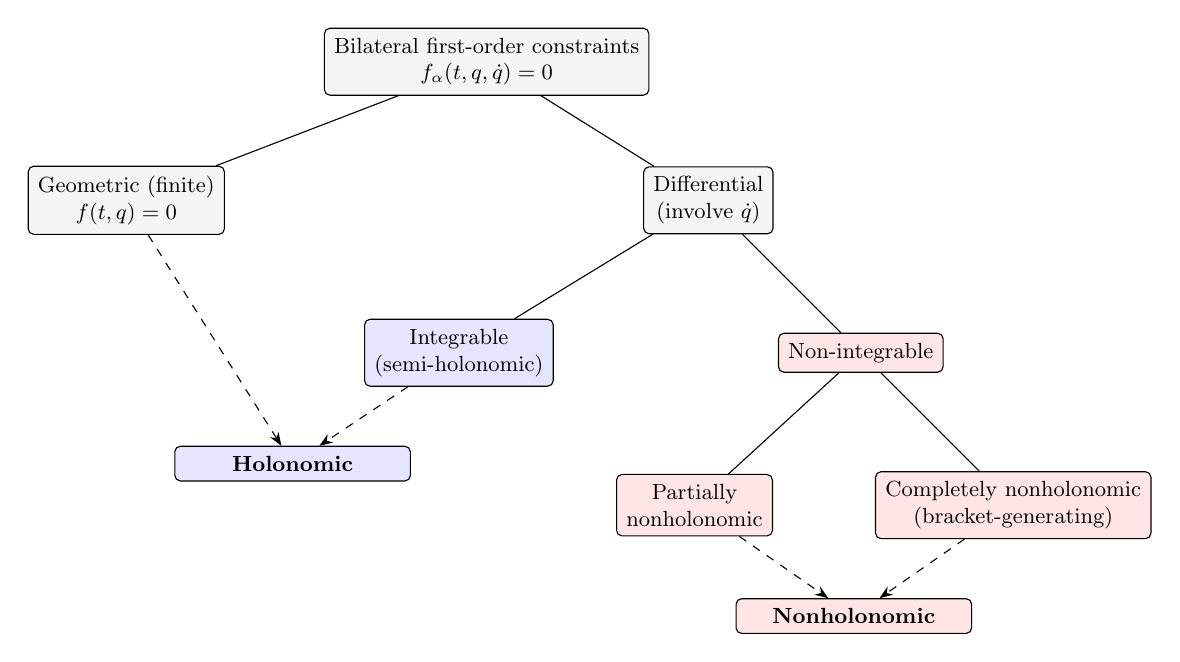
\begin{tikzpicture}[scale=0.88,transform shape,
    box/.style={draw,rounded corners=2pt,align=center,inner sep=4pt,font=\small,fill=gray!8},
    hol/.style={box,fill=blue!10},
    nonhol/.style={box,fill=red!10},
    >=Stealth,
    every edge/.style={draw,->}]
  \node[box] (root) at (0,0) {Bilateral first-order constraints\\ $f_\alpha(t,q,\dot q)=0$};
  \node[box] (geo)  at (-5.2,-2.0) {Geometric (finite)\\ $f(t,q)=0$};
  \node[box] (diff) at (3.2,-2.0) {Differential\\ (involve $\dot q$)};
  \node[hol] (int)  at (-0.4,-4.2) {Integrable\\ (semi-holonomic)};
  \node[nonhol] (non) at (5.4,-4.2) {Non-integrable};
  \node[nonhol] (part) at (3.0,-6.4) {Partially\\ nonholonomic};
  \node[nonhol] (comp) at (7.6,-6.4) {Completely nonholonomic\\ (bracket-generating)};
  \draw (root) -- (geo);
  \draw (root) -- (diff);
  \draw (diff) -- (int);
  \draw (diff) -- (non);
  \draw (non) -- (part);
  \draw (non) -- (comp);
  % brackets
  \node[hol,minimum width=3.4cm] (H) at (-2.8,-5.8) {\textbf{Holonomic}};
  \draw[->,dashed] (geo) -- (H);
  \draw[->,dashed] (int) -- (H);
  \node[nonhol,minimum width=3.4cm] (NH) at (5.3,-8.0) {\textbf{Nonholonomic}};
  \draw[->,dashed] (part) -- (NH);
  \draw[->,dashed] (comp) -- (NH);
\end{tikzpicture}
\caption{Hierarchy of bilateral first-order constraints. Orthogonally, differential
constraints may be linear homogeneous, affine, or nonlinear in $\dot q$, and
scleronomic or rheonomic.}\label{fig:tree}
\end{figure}

\begin{table}[t]
\centering
\small
\renewcommand{\arraystretch}{1.25}
\begin{tabular}{@{}p{2.9cm}p{3.6cm}p{5.0cm}p{3.1cm}@{}}
\toprule
\textbf{Criterion} & \textbf{Classes} & \textbf{Defining property} & \textbf{Typical example}\\
\midrule
Order & geometric / kinematic / dynamic & highest derivative in $f$: $0$ / $1$ / $\ge2$ & rigid rod / rolling / servo-constraint\\
Integrability & holonomic (incl.\ semi-holonomic) / nonholonomic & Frobenius: $\mathrm{d}\omega^\alpha\wedge\omega^1\wedge\dots\wedge\omega^m=0$ or not & pendulum / knife-edge\\
Velocity dependence & linear homogeneous / affine / nonlinear & form of $f$ in $\dot q$ & rolling disk / moving belt / constant-speed constraint\\
Time & scleronomic / rheonomic & $\partial f/\partial t=0$ or $\neq0$ & fixed hoop / rotating hoop\\
Sidedness & bilateral / unilateral & $f=0$ / $f\ge0$ & rod / string, wall\\
Reaction work & ideal / non-ideal & $\sum R_i\delta q^i=0$ or not & smooth wire / Coulomb friction\\
Regularity & regular / singular & $\rank\,\partial f/\partial q=m$ or not & circle / cusp\\
Phase space & primary / secondary; first / second class & Dirac's algorithm; $\Pois{\varphi_a}{\varphi_b}\weq0$ or not & relativistic particle / sphere\\
\bottomrule
\end{tabular}
\caption{Independent axes of classification of mechanical constraints.}\label{tab:classes}
\end{table}

% =====================================================================
\section{Geometry of differential constraints}\label{sec:geometry}
% =====================================================================
The question ``is this differential constraint secretly a finite relation?'' has a
complete, constructive answer in terms of Lie brackets. Throughout this section the
constraints are Pfaffian. To treat time dependence and inhomogeneous terms on the same
footing we work on the extended space $\R_t\times Q$ with the $1$-forms
\begin{equation}\label{eq:forms}
  \omega^\alpha=\sum_i a_{\alpha i}(q,t)\,\dd q^i+a_{\alpha 0}(q,t)\,\dd t,\qquad\alpha=1,\dots,m,
\end{equation}
assumed linearly independent. For the purely scleronomic homogeneous case we may
simply work on $Q$.

Let $\mathcal D_q=\bigcap_\alpha\ker\omega^\alpha_q\subset T_qQ$ be the
\emph{constraint distribution}, of rank $n-m$. Choosing a basis of vector fields,
$\mathcal D=\Span\{g_1,\dots,g_{n-m}\}$, the admissible velocities are exactly
\begin{equation}\label{eq:kinematic-control}
  \dot q=\sum_{r=1}^{n-m}u_r\,g_r(q),\qquad u_r\in\R,
\end{equation}
where the $u_r$ are \emph{quasi-velocities}. In control-theoretic language, \eqref{eq:kinematic-control} is a
driftless control system and the constraint is a statement about its controllability.

\begin{definition}[Lie bracket]
For vector fields $X,Y$ on $Q$ the Lie bracket is $[X,Y]^i=\sum_j\bigl(X^j\partial_jY^i-Y^j\partial_jX^i\bigr)$.
The distribution $\mathcal D$ is \emph{involutive} if $[X,Y]\in\mathcal D$ for all $X,Y\in\mathcal D$.
\end{definition}

\begin{theorem}[Frobenius]\label{thm:frobenius}
The following are equivalent:
\begin{enumerate}[label=(\roman*),leftmargin=2em]
  \item $\mathcal D$ is involutive, i.e.\ $[g_r,g_s]\in\Span\{g_1,\dots,g_{n-m}\}$ for all $r,s$;
  \item $\dd\omega^\alpha\wedge\omega^1\wedge\dots\wedge\omega^m=0$ for every $\alpha$;
  \item through every point passes an integral manifold of dimension $n-m$ (locally: there
        exist $m$ functions $f_\beta(q,t)$ with $\{\omega^\alpha=0\}\Longleftrightarrow\{\dd f_\beta=0\}$),
        so the constraints are holonomic.
\end{enumerate}
\end{theorem}

\begin{remark}[Single constraint in three dimensions]
For $m=1$, $n=3$, $\omega=\mathbf a\cdot\dd\mathbf q$, condition~(ii) is the classical
Euler criterion
\begin{equation}\label{eq:euler}
  \mathbf a\cdot(\nabla\times\mathbf a)=0,
\end{equation}
which says that an integrating factor $\mu(\mathbf q)$ exists with $\mu\,\mathbf a=\nabla f$.
\end{remark}

When \eqref{eq:euler} (or its general form) \emph{fails}, the failure is not merely a
technicality: following a small closed loop in the projected coordinates along admissible
curves leaves a net displacement in the transverse direction, proportional to the bracket
times the enclosed area. This is the mechanism by which a car can be parallel-parked
although it cannot move sideways.

\paragraph{The growth vector and Chow--Rashevskii.}
Define recursively $\mathcal D^1=\mathcal D$ and $\mathcal D^{k+1}=\mathcal D^k+[\mathcal D,\mathcal D^k]$.
The sequence of ranks $(\rank\mathcal D^1,\rank\mathcal D^2,\dots)$ is the \emph{growth vector}. The
limit $\mathcal D^\infty$ is the smallest involutive distribution containing $\mathcal D$.

\begin{theorem}[Chow--Rashevskii \cite{Chow1939}]\label{thm:chow}
If $\mathcal D^k_q=T_qQ$ for some $k$ at every $q$ of a connected manifold $Q$ (the
distribution is \emph{bracket-generating}), then any two points of $Q$ can be joined by an
admissible curve. More generally, the set reachable from $q$ by admissible curves is the
leaf of $\mathcal D^\infty$ through $q$.
\end{theorem}

This gives the refined classification of Section~\ref{sec:holo}:
\[
\begin{array}{lll}
\text{holonomic} & \iff \mathcal D^\infty=\mathcal D, & \text{leaf dimension } n-m,\\
\text{partially nonholonomic} & \iff \mathcal D\subsetneq\mathcal D^\infty\subsetneq TQ, & \text{leaf dimension } \rank\mathcal D^\infty,\\
\text{completely nonholonomic} & \iff \mathcal D^\infty=TQ, & \text{leaf dimension } n.
\end{array}
\]

% =====================================================================
\section{Equations of motion}\label{sec:dynamics}
% =====================================================================
\subsection{d'Alembert--Lagrange principle and Lagrange multipliers}\label{sec:dalembert}
Let $L(q,\dot q,t)=T-V$ and let $Q_i$ denote applied generalised forces not derived from
$V$. The \emph{d'Alembert--Lagrange principle} states that for \emph{ideal} constraints the
true motion satisfies
\begin{equation}\label{eq:dalembert}
  \sum_{i=1}^n\Bigl(\ddt\pd L{\dot q^i}-\pd L{q^i}-Q_i\Bigr)\delta q^i=0
  \qquad\forall\,\delta q\in\mathcal V_{(t,q)}.
\end{equation}
Because $\mathcal V_{(t,q)}=\{\delta q:\sum a_{\alpha i}\delta q^i=0\}$, the bracket must lie in the
span of the constraint gradients, which gives the \emph{Lagrange equations of the first kind}
\begin{equation}\label{eq:lagrange-first}
  \boxed{\;\ddt\pd L{\dot q^i}-\pd L{q^i}=Q_i+\sum_{\alpha=1}^m\lambda_\alpha\,a_{\alpha i}(q,t),
  \qquad i=1,\dots,n,\;}
\end{equation}
together with the $m$ constraint equations \eqref{eq:pfaffian}. The $n+m$ equations determine
the $n$ functions $q^i(t)$ and the $m$ multipliers $\lambda_\alpha(t)$. The constraint force
is $R_i=\sum_\alpha\lambda_\alpha a_{\alpha i}$; in particular the multipliers carry
direct physical meaning (tensions, normal forces). For a holonomic constraint $f_\beta(q,t)=0$
one has $a_{\beta i}=\partial f_\beta/\partial q^i$.

\paragraph{Holonomic reduction.} If all constraints are holonomic one can eliminate
the multipliers \emph{a priori}: choose $n-m$ independent coordinates $s=(s^1,\dots,s^{n-m})$
with $q=q(s,t)$ solving $f_\beta=0$, substitute into $L$ to obtain $\tilde L(s,\dot s,t)$, and
write the ordinary Lagrange equations
$\ddt\partial\tilde L/\partial\dot s^r-\partial\tilde L/\partial s^r=\tilde Q_r$ with no reactions at all.
This is the standard route and the main practical benefit of holonomic constraints.

\subsection{Explicit solution for the multipliers; Gauss's principle}\label{sec:gauss}
For a natural system $L=\tfrac12\dot q\transp M(q)\dot q-V(q)$ with positive-definite mass
matrix $M$, write \eqref{eq:lagrange-first} as
\begin{equation}\label{eq:dae}
  M\ddot q=F(q,\dot q,t)+A\transp\lambda,\qquad A\ddot q=-\dot A\dot q-\dot b\;\equiv\;c(q,\dot q,t),
\end{equation}
where $F$ collects applied, potential, Coriolis and centrifugal forces and the second
equation is the time derivative of $A\dot q+b=0$. If $A$ has full row rank, $AM^{-1}A\transp$
is invertible and
\begin{equation}\label{eq:lambda}
  \lambda=\bigl(AM^{-1}A\transp\bigr)^{-1}\bigl(c-AM^{-1}F\bigr),\qquad
  \ddot q=M^{-1}F+M^{-1}A\transp\lambda.
\end{equation}
This is an explicit ODE for $q$; it is the Udwadia--Kalaba form \cite{UdwadiaKalaba1992}
(with a pseudo-inverse when the constraints are redundant).

Equation \eqref{eq:lambda} has a variational meaning. Define the \emph{constraint measure}
\begin{equation}\label{eq:gauss}
  Z(\ddot q)=\tfrac12\bigl(\ddot q-M^{-1}F\bigr)\transp M\bigl(\ddot q-M^{-1}F\bigr)
  =\tfrac12\sum_i m_i\Bigl|\ddot{\mathbf r}_i-\frac{\mathbf F_i}{m_i}\Bigr|^2 .
\end{equation}

\begin{theorem}[Gauss's principle of least constraint, 1829 \cite{Gauss1829}]
At each instant, among all accelerations compatible with the constraints (for \eqref{eq:pfaffian},
those satisfying $A\ddot q=c$), the actual acceleration is the one that minimises $Z$.
\end{theorem}

The constrained acceleration is thus the free acceleration $M^{-1}F$ orthogonally
projected, in the metric $M$, onto the affine set of admissible accelerations. The principle
applies verbatim to unilateral constraints (the minimisation becomes a quadratic program),
to nonlinear constraints, and to dynamic constraints (Section~\ref{sec:classification}).

\subsection{Quasi-velocities: Maggi, Gibbs--Appell, Chaplygin}
For nonholonomic systems it is often preferable to avoid multipliers altogether. Choose
quasi-velocities $\pi_r$ ($r=1,\dots,n-m$) parametrising admissible velocities,
$\dot q^i=\sum_rB_{ir}(q,t)\pi_r+\beta_i(q,t)$, as in \eqref{eq:kinematic-control}.
Then:
\begin{itemize}[leftmargin=1.2em]
\item \textbf{Maggi's equations.} Projecting \eqref{eq:dalembert} onto the columns of $B$,
\[
  \sum_iB_{ir}\Bigl(\ddt\pd L{\dot q^i}-\pd L{q^i}-Q_i\Bigr)=0,\qquad r=1,\dots,n-m.
\]
\item \textbf{Gibbs--Appell equations.} With the acceleration energy
$S=\tfrac12\sum_im_i|\ddot{\mathbf r}_i|^2$ expressed as a function of the quasi-accelerations
$\dot\pi_r$,
\begin{equation}\label{eq:appell}
  \pd S{\dot\pi_r}=\Pi_r,\qquad r=1,\dots,n-m,
\end{equation}
where $\Pi_r=\sum_i(Q_i-\partial V/\partial q^i)B_{ir}$ are the generalised forces conjugate to
the quasi-velocities \cite{Gibbs1879,Pars1965}. No multipliers appear and the constraints
need not be differentiated. (The equations \eqref{eq:appell} are equivalent to Gauss's principle.)
\item \textbf{Chaplygin systems.} If the constraints and $L$ are invariant under the
shifts of some of the coordinates ($q=(s,y)$ with constraints $\dot y=B(s)\dot s$ and $L$
independent of $y$), one obtains a \emph{reduced} system in $s$ alone. The reduced
equations are Lagrange equations of the constrained Lagrangian plus a gyroscopic-type term
proportional to the curvature of the constraint \cite{Bloch1996,Bloch2003}.
\end{itemize}

\subsection{Nonlinear constraints and Chetaev's condition}\label{sec:chetaev}
For $f_\alpha(t,q,\dot q)=0$ nonlinear in $\dot q$, d'Alembert's principle must be supplemented
by a rule specifying which displacements are virtual. \emph{Chetaev's condition}
\eqref{eq:chetaev} postulates that the reaction is a combination of the velocity gradients,
\begin{equation}\label{eq:chetaev-eom}
  \ddt\pd L{\dot q^i}-\pd L{q^i}=Q_i+\sum_\alpha\lambda_\alpha\pd{f_\alpha}{\dot q^i}.
\end{equation}
Gauss's principle applied to the once-differentiated constraint gives exactly the same
equations, so the two are consistent. It is important to stress that Chetaev's condition is a
\emph{postulate about the reactions}: for linear constraints it is forced by d'Alembert's
principle, but for nonlinear constraints its applicability to a concrete physical device has
to be justified separately (this point was already discussed by Appell and
Hamel; see \cite{NeimarkFufaev1972}).

\subsection{Nonholonomic versus vakonomic mechanics}\label{sec:vako}
There is an alternative, variational, way to treat nonholonomic constraints: impose the
constraint on the competing paths \emph{before} varying the action. For Pfaffian constraints
this leads, with multipliers $\mu_\alpha(t)$, to the Euler--Lagrange equations of
$L^*=L+\sum_\alpha\mu_\alpha\sum_ia_{\alpha i}\dot q^i$:
\begin{equation}\label{eq:vakonomic}
  \ddt\Bigl(\pd L{\dot q^i}+\sum_\alpha\mu_\alpha a_{\alpha i}\Bigr)-\pd L{q^i}-\sum_{\alpha,j}\mu_\alpha\pd{a_{\alpha j}}{q^i}\dot q^j=0 .
\end{equation}
This is called \emph{vakonomic} mechanics (variational axiomatic kind; Arnold and Kozlov). Compare with
\eqref{eq:lagrange-first}: in the \emph{holonomic} case ($a_{\alpha i}=\partial_if_\alpha$) the
extra terms in \eqref{eq:vakonomic} reduce, because $\partial_ia_{\alpha j}=\partial_ja_{\alpha i}$, to $\dot\mu_\alpha a_{\alpha i}$, and the two systems are
equivalent with $\lambda_\alpha=-\dot\mu_\alpha$. For \emph{nonintegrable} constraints they differ,
and the difference is real (Example~\ref{ex:heisenberg}). The d'Alembert--Lagrange model
\eqref{eq:lagrange-first} describes rolling and sliding contacts realised, for instance, by
strong friction forces; the vakonomic model describes optimal-control problems (sub-Riemannian
geodesics) and a different limiting realisation of the constraint \cite{Kozlov1983,AKN2006}.
Also note that the vakonomic equations are of higher order: the multipliers are dynamical variables whose
initial values are additional data, so the evolution is not determined by $(q,\dot q)$ alone.

\subsection{Unilateral constraints and complementarity}\label{sec:unilateral}
Let the unilateral constraints be $g_j(q,t)\ge0$, $j\in J$. The equations of motion are
\begin{equation}\label{eq:signorini}
  M\ddot q=F+\sum_{j\in J}\lambda_j\nabla g_j,\qquad
  0\le\lambda_j\ \compl\ g_j\ge0 ,
\end{equation}
where $x\compl y$ means $xy=0$ (the Signorini conditions): either the constraint is
inactive ($g_j>0$, no force) or it is active ($g_j=0$, $\lambda_j\ge0$, i.e.\ push only).
At the acceleration level, for contacts that are active and have $\dot g_j=0$, the
condition becomes $0\le\lambda_j\compl\ddot g_j\ge0$. Inserting $\ddot g=G\ddot q+\gamma$
($G=\partial g/\partial q$) and $\ddot q$ from the equation of motion gives a
\emph{linear complementarity problem} (LCP) for the active multipliers,
\begin{equation}\label{eq:lcp}
  \ddot g=W\lambda+w,\quad W=GM^{-1}G\transp,\quad 0\le\lambda\ \compl\ \ddot g\ge0,
\end{equation}
which has a unique solution whenever $G$ has full row rank (since then $W\succ0$); this
is the same as Gauss's principle with inequality constraints.
When the approach velocity is nonzero at $g_j=0$, an \emph{impact} occurs: the velocity is
discontinuous, $M(\dot q^+-\dot q^-)=\sum_j\Lambda_j\nabla g_j$ with impulses $\Lambda_j\ge0$,
closed by a restitution law such as Newton's $\dot g_j^+=-e\,\dot g_j^-$, $0\le e\le1$.
See \cite{Moreau1988,PfeifferGlocker1996,Brogliato2016} for the full non-smooth theory.

\subsection{Non-ideal constraints: friction}\label{sec:friction}
For a non-ideal constraint the reaction is $\mathbf R=N\hat{\mathbf n}+\mathbf T$ with
tangential component $\mathbf T$ that does virtual work and must be given by a
constitutive law. With Coulomb's law,
\begin{equation}\label{eq:coulomb}
  \text{stick: }\ \mathbf v_t=0,\ |\mathbf T|\le\mu_sN;\qquad
  \text{slip: }\ \mathbf v_t\ne0,\ \mathbf T=-\mu_kN\,\frac{\mathbf v_t}{|\mathbf v_t|},
\end{equation}
where $\mathbf v_t$ is the tangential relative velocity. Coulomb friction can make the
LCP \eqref{eq:lcp} nonsymmetric (the matrix $W$ is no longer positive definite), and
rigid-body models can then admit no solution or several (the \emph{Painlev\'e paradoxes}
\cite{Brogliato2016}).

% =====================================================================
\section{Hamiltonian constraints: Dirac's classification}\label{sec:dirac}
% =====================================================================
The constraints of the previous sections restrict $(q,\dot q)$. A different kind of
constraint arises when the Lagrangian is \emph{singular}, that is, when the Hessian
$W_{ij}=\partial^2L/\partial\dot q^i\partial\dot q^j$ has rank $n-k<n$. Then the Legendre map
$\dot q\mapsto p=\partial L/\partial\dot q$ is not invertible and the momenta satisfy $k$
relations independent of velocities \cite{Dirac1950,Dirac1964,HenneauxTeitelboim1992}.

\subsection{Dirac's algorithm}
\begin{enumerate}[leftmargin=1.6em]
\item \textbf{Primary constraints.} The relations $\varphi_m(q,p)\weq0$, $m=1,\dots,k$, that
  follow from the definition of the momenta. Here $\weq$ denotes \emph{weak equality}
  (equality on the constraint surface, to be imposed only after all Poisson brackets have been
  evaluated).
\item \textbf{Total Hamiltonian.} With the canonical Hamiltonian
  $H_c=\sum p_i\dot q^i-L$ (well defined on the primary surface),
  \begin{equation}\label{eq:HT}
    H_T=H_c+\sum_{m}u^m(t)\,\varphi_m,\qquad \dot F\weq\Pois F{H_T},
  \end{equation}
  with arbitrary multipliers $u^m$.
\item \textbf{Consistency.} Primary constraints must be preserved in time:
  \[
    \dot\varphi_m\weq\Pois{\varphi_m}{H_c}+\sum_{m'}u^{m'}\Pois{\varphi_m}{\varphi_{m'}}\weq0 .
  \]
  Each such condition either (a) fixes some of the $u^m$, (b) is identically satisfied, or
  (c) yields a new relation among $(q,p)$, a \emph{secondary constraint}. The procedure is
  iterated on the new constraints (giving tertiary constraints, etc.) until no further
  independent relations appear.
\end{enumerate}
The \emph{primary/secondary} distinction thus reflects the \emph{origin} of a constraint
(directly from the Legendre map, or from consistency).

\begin{definition}[First- and second-class]
A phase-space function $F$ is \emph{first class} if $\Pois F{\varphi_a}\weq0$ for all
constraints $\varphi_a$ of the complete set, and \emph{second class} otherwise. Each constraint
can be replaced by independent combinations so that the complete set splits into $N_1$
first-class constraints $\gamma_A$ and $N_2$ second-class constraints $\chi_\mu$; the
matrix $C_{\mu\nu}=\Pois{\chi_\mu}{\chi_\nu}$ is then invertible (in particular $N_2$ is even).
\end{definition}

\begin{description}[leftmargin=1.2em,style=nextline]
\item[Second-class constraints] are eliminated with the \emph{Dirac bracket}
  \begin{equation}\label{eq:dirac-bracket}
    \Pois FG_D=\Pois FG-\sum_{\mu,\nu}\Pois F{\chi_\mu}\,(C^{-1})^{\mu\nu}\,\Pois{\chi_\nu}G ,
  \end{equation}
  which satisfies the Jacobi identity, and for which $\Pois F{\chi_\mu}_D=0$ for all $F$.
  Constraints can then be set strongly equal to zero.
\item[First-class constraints] generate \emph{gauge transformations}
  $\delta F=\sum_A\epsilon^A(t)\Pois F{\gamma_A}$ (for primary first-class constraints this
  is the statement that the corresponding $u^m$ remain arbitrary; for the secondary ones it is
  Dirac's conjecture, which holds in all physically relevant cases but is not a theorem in
  complete generality \cite{HenneauxTeitelboim1992}). The equations of motion contain
  arbitrary functions of time, and the physical state space is the reduced space obtained by
  quotienting by the gauge orbits.
\end{description}
The number of physical degrees of freedom is
\begin{equation}\label{eq:dof}
  \underbrace{n}_{\text{coordinates}}-\,N_1-\tfrac12N_2 .
\end{equation}

\subsection{Relation to kinematic constraints}
A holonomic constraint $f(q)=0$ on a natural system with $H=\tfrac12p\transp M^{-1}p+V$ may
be imposed as a phase-space constraint $\varphi_1=f\weq0$. Consistency yields the secondary
constraint $\varphi_2=\nabla f\transp M^{-1}p\weq0$ (the velocity is tangent), and
$\Pois{\varphi_1}{\varphi_2}=\nabla f\transp M^{-1}\nabla f\neq0$. The pair is second class.
The Dirac bracket \eqref{eq:dirac-bracket} is the canonical Poisson bracket of
the cotangent bundle $T^*\{f=0\}$ of the constraint manifold.

For \emph{nonholonomic} constraints the situation is qualitatively different. Writing the
constraints as linear conditions on the momenta, one still obtains a well-defined
bracket on the constraint submanifold of $T^*Q$ for the d'Alembert--Lagrange dynamics, but it is
only \emph{almost Poisson}: it is skew-symmetric and satisfies the Leibniz rule, but it
violates the Jacobi identity, and by a result of van der Schaft and Maschke it satisfies it
iff the constraints are integrable \cite{vdSchaftMaschke1994}. Nonholonomic dynamics is therefore
not Hamiltonian in the strict sense: it does not preserve a symplectic form on the constraint
manifold, though the energy is conserved for scleronomic homogeneous constraints.

\begin{example}[Free relativistic particle: first class]\label{ex:relparticle}
Let $L=-mc\sqrt{-\eta_{\mu\nu}\dot x^\mu\dot x^\nu}$, signature $(-,+,+,+)$, $x^0=ct$, with
dots denoting derivatives with respect to an \emph{arbitrary} parameter $\tau$. Then
$p_\mu=mc\,\eta_{\mu\nu}\dot x^\nu/\sqrt{-\dot x\cdot\dot x}$ satisfies identically
\[
  \varphi\equiv\eta^{\mu\nu}p_\mu p_\nu+m^2c^2\weq0 .
\]
This is the mass-shell condition; it is the single primary constraint. The canonical
Hamiltonian vanishes identically ($L$ is homogeneous of degree one in the velocities), so
$H_T=u(\tau)\,\varphi$. Consistency, $\dot\varphi\weq u\Pois\varphi\varphi=0$, holds
automatically, so $\varphi$ is first class. The equations of motion are
$\dot x^\mu=2u\,p^\mu$, $\dot p_\mu=0$, in which $u(\tau)$ is arbitrary: this is the
reparametrisation freedom $\tau\to\tau'(\tau)$. The phase space has dimension $8$;
$N_1=1$ removes $2$, leaving the $6$-dimensional physical phase space $(\mathbf x,\mathbf p)$ of
a free particle. Gauge fixing $x^0=c\tau$ returns the usual dynamics.
\end{example}

\begin{example}[Particle on a sphere: second class]\label{ex:sphere}
Let $H=\mathbf p^2/2m+V(\mathbf x)$ with the constraint $\varphi_1=\mathbf x^2-R^2\weq0$.
Consistency gives $\varphi_2=\mathbf x\cdot\mathbf p\weq0$, and
$\Pois{\varphi_1}{\varphi_2}=2\mathbf x^2\weq2R^2\ne0$: the pair is second class. Consistency of
$\varphi_2$ then \emph{fixes} the multiplier of $\varphi_1$,
$u=(\mathbf p^2/m-\mathbf x\cdot\nabla V)/(2R^2)$, so $\dot{\mathbf p}=-\nabla V-2u\mathbf x$
contains the centripetal reaction and there is no gauge freedom. With
$C_{12}=-C_{21}=2R^2$, \eqref{eq:dirac-bracket} gives
\[
  \Pois{x_i}{x_j}_D=0,\qquad
  \Pois{x_i}{p_j}_D=\delta_{ij}-\frac{x_ix_j}{R^2},\qquad
  \Pois{p_i}{p_j}_D=-\frac{x_ip_j-x_jp_i}{R^2},
\]
i.e.\ the bracket projects onto the tangent plane of the sphere. Here $N_2=2$, $N_1=0$,
$n=3$, and \eqref{eq:dof} gives $2$ physical degrees of freedom.
\end{example}

\begin{example}[Toy gauge system]\label{ex:toygauge}
$L=\tfrac12(\dot q^1-\dot q^2)^2$. Then $p_1=-p_2=\dot q^1-\dot q^2$ and there is one
primary constraint $\varphi=p_1+p_2\weq0$, with $H_c=\tfrac12p_1^2$. Since $H_c$ and
$\varphi$ do not depend on $q$, $\Pois\varphi{H_c}=0$: no secondary constraints, and $\varphi$
is first class. Only the difference $q^1-q^2$ is physical; $q^1+q^2$ is pure gauge. By
\eqref{eq:dof}, $n-N_1=1$ physical degree of freedom.
\end{example}

% =====================================================================
\section{A catalogue of examples}\label{sec:examples}
% =====================================================================
Each example is tagged with its classification. Table~\ref{tab:examples} at the end of the
section collects the results.

\subsection{Holonomic constraints}

\begin{example}[Simple pendulum --- holonomic, scleronomic, bilateral, ideal]\label{ex:pendulum}
A bob of mass $m$ in the plane $(x,y)$ ($y$ up), $f=x^2+y^2-\ell^2=0$, $L=\tfrac12m(\dot x^2+\dot y^2)-mgy$.
Equations \eqref{eq:lagrange-first} with $a=\nabla f=(2x,2y)$:
\[
  m\ddot x=2\lambda x,\qquad m\ddot y=-mg+2\lambda y .
\]
With $x=\ell\sin\theta$, $y=-\ell\cos\theta$, elimination of the constraint gives
$\ddot\theta+(g/\ell)\sin\theta=0$, while the radial component yields the tension
\[
  T=-2\lambda\ell=mg\cos\theta+m\ell\dot\theta^2 .
\]
If the bob hangs from a \emph{string} instead of a rod the constraint is unilateral,
$f\le0$, and the requirement $T\ge0$ must be monitored: the string goes slack, and the motion
becomes that of a free projectile, when $T$ reaches zero.
\end{example}

\begin{example}[Bead on a rotating hoop --- holonomic, \emph{rheonomic}]\label{ex:hoop}
A bead slides without friction on a circular hoop of radius $R$ that rotates with constant
angular velocity $\omega$ about a vertical diameter. In Cartesian coordinates the two
constraints are $\mathbf x^2=R^2$ (scleronomic) and $y\cos\omega t-x\sin\omega t=0$
(rheonomic). With $\theta$ measured from the downward vertical,
\[
  \tilde L=\tfrac12mR^2\bigl(\dot\theta^2+\omega^2\sin^2\theta\bigr)+mgR\cos\theta,\qquad
  \ddot\theta=\sin\theta\Bigl(\omega^2\cos\theta-\frac gR\Bigr).
\]
For $\omega^2<g/R$ the only stable equilibrium is $\theta=0$; at $\omega^2=g/R$ it
loses stability in a pitchfork bifurcation to $\cos\theta_0=g/(R\omega^2)$. The Jacobi integral
\[
  h=\tfrac12mR^2\dot\theta^2-\tfrac12mR^2\omega^2\sin^2\theta-mgR\cos\theta
\]
is conserved, but the energy $E=T+V=h+mR^2\omega^2\sin^2\theta$ is \emph{not}. The
normal reaction of the hoop has an azimuthal component (Coriolis) that does work on the real
displacement, although it does no virtual work: the constraint is ideal, yet not
workless. This illustrates the difference between virtual and actual displacement
(Section~\ref{sec:virtual}).
\end{example}

\begin{example}[Rigid body --- internal holonomic constraints]\label{ex:rigid}
A rigid body of $N\ge3$ non-collinear particles obeys $|\mathbf r_i-\mathbf r_j|^2=d_{ij}^2$.
Only $3N-6$ of these are independent, so the body has $6$ degrees of freedom (position of
a reference point plus three orientation angles). A dumbbell (two masses on a rigid massless rod) has one
constraint and $5$ degrees of freedom. The reactions are $\mathbf R_1=-\mathbf R_2=\lambda(\mathbf r_1-\mathbf r_2)$,
which do no virtual work, $\mathbf R_1\cdot\delta\mathbf r_1+\mathbf R_2\cdot\delta\mathbf r_2
=\lambda(\mathbf r_1-\mathbf r_2)\cdot(\delta\mathbf r_1-\delta\mathbf r_2)=0$. The constraint is
ideal.
\end{example}

\begin{example}[Particle on a hemisphere --- unilateral]\label{ex:hemisphere}
A particle starts at rest (with negligible perturbation) at the top of a smooth fixed sphere of radius
$R$, with constraint $g=r-R\ge0$ and multiplier $\lambda=N\ge0$. While in contact,
energy conservation gives $v^2=2gR(1-\cos\theta)$ and the radial equation gives
\[
  N=mg\cos\theta-\frac{mv^2}R=mg\,(3\cos\theta-2).
\]
The Signorini condition $N\ge0$ is violated for $\cos\theta<2/3$: the particle leaves the
surface at $\theta_c=\arccos(2/3)\approx48.2^\circ$ with $v^2=\tfrac23gR$ and continues as a
free projectile. The constraint switches from active to inactive at an event
determined by $\lambda=0$.
\end{example}

\subsection{Semi-holonomic: an integrable differential constraint}

\begin{example}[Cylinder rolling down an incline --- semi-holonomic]\label{ex:cylinder}
Let a homogeneous cylinder ($I=\tfrac12mR^2$) roll without slipping down an incline of angle
$\alpha$. With $x$ the distance along the slope and $\varphi$ the rotation angle,
$L=\tfrac12m\dot x^2+\tfrac12I\dot\varphi^2+mgx\sin\alpha$. The no-slip condition is
the Pfaffian constraint $\dot x-R\dot\varphi=0$, i.e.\ $a=(1,-R)$. It looks
nonholonomic but is integrable: $x-R\varphi=\text{const}$ (indeed $\omega=\dd x-R\,\dd\varphi$
is exact). The multiplier equations
\[
  m\ddot x-mg\sin\alpha=\lambda,\qquad I\ddot\varphi=-R\lambda
\]
give $\ddot x=\tfrac23g\sin\alpha$ and $\lambda=-\tfrac13mg\sin\alpha$, which is the static
friction force; it is feasible iff $\mu_s\ge\tfrac13\tan\alpha$.
\end{example}

\subsection{Nonholonomic constraints}

\begin{example}[Vertical disk rolling on a plane --- completely nonholonomic]\label{ex:disk}
A thin disk of radius $R$ stays upright and rolls without slipping on a horizontal plane. Coordinates
are $q=(x,y,\theta,\varphi)$: contact point $(x,y)$, heading angle $\theta$, rolling
angle $\varphi$. The velocity of the contact point of the disk with the ground is zero:
\[
  \dot x=R\dot\varphi\cos\theta,\qquad \dot y=R\dot\varphi\sin\theta,
\]
i.e.\ $\omega^1=\dd x-R\cos\theta\,\dd\varphi$, $\omega^2=\dd y-R\sin\theta\,\dd\varphi$.
These are linear homogeneous scleronomic. Non-integrability follows from Frobenius' condition:
\[
  \dd\omega^1\wedge\omega^1\wedge\omega^2=R\sin\theta\;\dd x\wedge\dd y\wedge\dd\theta\wedge\dd\varphi,\quad
  \dd\omega^2\wedge\omega^1\wedge\omega^2=-R\cos\theta\;\dd x\wedge\dd y\wedge\dd\theta\wedge\dd\varphi,
\]
which cannot both vanish. A basis of the distribution is
$g_1=R\cos\theta\,\partial_x+R\sin\theta\,\partial_y+\partial_\varphi$, $g_2=\partial_\theta$, and
$[g_2,g_1]=-R\sin\theta\,\partial_x+R\cos\theta\,\partial_y=:g_3$,
$[g_2,g_3]=-R(\cos\theta\,\partial_x+\sin\theta\,\partial_y)$. Hence $g_1,g_2,g_3,[g_2,g_3]$ span
$T_qQ$: the growth vector is $(2,3,4)$, the system is completely nonholonomic, and
(Theorem~\ref{thm:chow}) any configuration can be reached from any other, although there are
only $n-m=2$ velocity degrees of freedom.

With the kinetic energy $T=\tfrac12m(\dot x^2+\dot y^2)+\tfrac12I_a\dot\varphi^2+\tfrac12I_d\dot\theta^2$ ($I_a$: moment about
the axle; $I_d$: moment about a vertical diameter), \eqref{eq:lagrange-first} reads
\[
  m\ddot x=\lambda_1,\quad m\ddot y=\lambda_2,\quad
  I_a\ddot\varphi=-R\bigl(\lambda_1\cos\theta+\lambda_2\sin\theta\bigr),\quad I_d\ddot\theta=0 .
\]
Differentiating the constraints gives $\ddot x\cos\theta+\ddot y\sin\theta=R\ddot\varphi$, hence
$\lambda_1\cos\theta+\lambda_2\sin\theta=mR\ddot\varphi$ and $(I_a+mR^2)\ddot\varphi=0$. Therefore
$\dot\varphi$ and $\dot\theta$ are constant: the contact point moves with constant speed
along a straight line ($\dot\theta=0$) or a circle of radius $R\dot\varphi/|\dot\theta|$.
\end{example}

\begin{example}[Knife edge, Chaplygin sleigh, and the kinematic car]\label{ex:sleigh}
A rigid body on a plane is supported by a blade (or wheel) at point $P=(x,y)$ that cannot
move laterally: $\dot x\sin\theta-\dot y\cos\theta=0$. With $\mathbf a=(\sin\theta,-\cos\theta,0)$
in $(x,y,\theta)$-space, $\mathbf a\cdot(\nabla\times\mathbf a)=-1\ne0$: the constraint is nonholonomic
\eqref{eq:euler}. The distribution is spanned by $g_1=\cos\theta\,\partial_x+\sin\theta\,\partial_y$ (roll)
and $g_2=\partial_\theta$ (pivot), with $[g_2,g_1]=-\sin\theta\,\partial_x+\cos\theta\,\partial_y$
(the forbidden sideways direction), so the growth vector is $(2,3)$. A cycle of four
motions (roll, turn, roll back, turn back) of duration $\varepsilon$ produces a net sideways
displacement $\varepsilon^2[g_1,g_2]+O(\varepsilon^3)$: this is parallel parking. The
same constraint describes the kinematic car $\dot x=v\cos\theta$, $\dot y=v\sin\theta$,
$\dot\theta=(v/L)\tan\psi$, with $v$ and the steering angle $\psi$ as controls.

For the \emph{Chaplygin sleigh} (mass $m$, moment of inertia $I$ about the centre of mass $C$,
blade at $P$ at distance $a$ behind $C$ on the axis of symmetry), let $u$ be the speed of $P$
along the heading. The velocity of $C$ is $u\,\mathbf e+a\dot\theta\,\mathbf n$, and the single lateral
reaction $F\mathbf n$ at $P$ gives
\begin{equation}\label{eq:sleigh}
  \dot u=a\dot\theta^2,\qquad (I+ma^2)\ddot\theta=-mau\dot\theta .
\end{equation}
The energy $E=\tfrac12m(u^2+a^2\dot\theta^2)+\tfrac12I\dot\theta^2$ is conserved,
$\dot E=mua\dot\theta^2+(I+ma^2)\dot\theta\ddot\theta=0$, as expected for a scleronomic homogeneous
constraint. Equation \eqref{eq:sleigh} is a closed system in $(u,\dot\theta)$ (a Chaplygin reduction: the
system is invariant under planar rigid motions), and for $u(0)>0$ one finds $\dot\theta\to0$, i.e.\ the sleigh
asymptotically travels in a straight line.
\end{example}

\begin{example}[Heisenberg system --- nonholonomic versus vakonomic]\label{ex:heisenberg}
Consider a free particle $L=\tfrac m2(\dot x^2+\dot y^2+\dot z^2)$ subject to the single
constraint $\dot z=x\dot y$, $\omega=\dd z-x\,\dd y$, $a=(0,-x,1)$. Since $\omega\wedge\dd\omega=-\dd z\wedge\dd x\wedge\dd y\neq0$,
the constraint is nonholonomic; $g_1=\partial_x$, $g_2=\partial_y+x\partial_z$, $[g_1,g_2]=\partial_z$,
growth vector $(2,3)$. Admissible curves satisfy $\Delta z=\oint x\,\dd y$, the area enclosed by the projection
onto the $(x,y)$-plane (the isoperimetric problem of Dido).

\emph{d'Alembert--Lagrange:} \eqref{eq:lagrange-first} reads $m\ddot x=0$, $m\ddot y=-\lambda x$,
$m\ddot z=\lambda$. Differentiating the constraint gives $\lambda=m\dot x\dot y/(1+x^2)$, so
$x=x_0+vt$ and $\dot y=C/\sqrt{1+x^2}$.

\emph{Vakonomic:} \eqref{eq:vakonomic} reads $m\ddot x=-\mu\dot y$, $m\dot y-\mu x=c_2$, $m\dot z+\mu=c_1$, so
$\mu=c_1-mx\dot y$ and $m\dot y(1+x^2)=c_2+c_1x$. Now $\ddot x\neq0$ in general.

Take the initial data $x=0$, $\dot x=0$, $\dot y=1$ ($m=1$). The d'Alembert motion is $x\equiv0$, $y=t$,
$z=0$. In vakonomic mechanics $\ddot x(0)=-\mu(0)$, where $\mu(0)$ is \emph{free initial
data}: there is a one-parameter family of motions with the same initial position and velocity,
and only $\mu(0)=0$ reproduces the d'Alembert solution. The two theories are genuinely different.
\end{example}

\begin{example}[Nonlinear constraint: the isokinetic constraint]\label{ex:isokinetic}
Constrain $N$ particles to constant kinetic energy,
$f=\tfrac12\sum_jm_j|\mathbf v_j|^2-K=0$. This is a scleronomic nonlinear
nonholonomic constraint (nonlinear in the velocities, and non-integrable except trivially). With $\partial f/\partial\mathbf v_i=m_i\mathbf v_i$,
Chetaev's condition \eqref{eq:chetaev-eom} gives $m_i\mathbf a_i=\mathbf F_i+\lambda m_i\mathbf v_i$.
Differentiating $f=0$ in time ($\sum m_i\mathbf v_i\cdot\mathbf a_i=0$) gives
\[
  m_i\mathbf a_i=\mathbf F_i-\alpha\,m_i\mathbf v_i,\qquad
  \alpha=\frac{\sum_j\mathbf F_j\cdot\mathbf v_j}{\sum_jm_j|\mathbf v_j|^2}.
\]
The reaction $-\alpha m_i\mathbf v_i$ is parallel to the velocity and does work
$-\sum_j\mathbf F_j\cdot\mathbf v_j$ on the real motion, exactly cancelling the power of the applied forces.
Thus an ideal (Chetaev) constraint can do work on the actual motion. This is Gauss's isokinetic
thermostat of nonequilibrium molecular dynamics \cite{EvansMorriss1990}. It is time-reversible but not Hamiltonian.
\end{example}

\subsection{Non-ideal constraints}

\begin{example}[Block on a rough incline --- friction]\label{ex:friction}
A block on an incline of angle $\alpha$: the surface is an ideal unilateral constraint with
reaction $N=mg\cos\alpha\ge0$, supplemented by the Coulomb law \eqref{eq:coulomb} for the tangential reaction
$T$. The block stays at rest iff $\tan\alpha\le\mu_s$ and otherwise slides with
$a=g(\sin\alpha-\mu_k\cos\alpha)$. The reaction $T$ does virtual work on displacements
along the plane, so the total reaction is a non-ideal constraint force: it cannot be written as
$\sum\lambda_\alpha a_{\alpha i}$, and in particular does not follow from multipliers alone.
\end{example}

\begin{table}[t]
\centering
\small
\renewcommand{\arraystretch}{1.2}
\begin{tabular}{@{}lllllcc@{}}
\toprule
\textbf{Example} & \textbf{Integrability} & \textbf{Time} & \textbf{Sides} & \textbf{Ideal} & $n$ & vel.\ d.o.f.\\
\midrule
Pendulum (rod)              & holonomic            & scleronomic & bilateral  & yes & 2 & 1\\
Pendulum (string)           & holonomic            & scleronomic & unilateral & yes & 2 & 1/2\\
Rotating hoop               & holonomic            & rheonomic   & bilateral  & yes & 3 & 1\\
Rigid body                  & holonomic            & scleronomic & bilateral  & yes & $3N$ & 6\\
Hemisphere                  & holonomic            & scleronomic & unilateral & yes & 3 & 2/3\\
Rolling cylinder            & semi-holonomic       & scleronomic & bilateral  & yes & 2 & 1\\
Vertical rolling disk       & completely nonhol.   & scleronomic & bilateral  & yes & 4 & 2\\
Knife edge / sleigh         & completely nonhol.   & scleronomic & bilateral  & yes & 3 & 2\\
Heisenberg system           & completely nonhol.   & scleronomic & bilateral  & yes & 3 & 2\\
Isokinetic constraint       & nonhol., nonlinear   & scleronomic & bilateral  & Chetaev & $3N$ & $3N-1$\\
Block with friction         & holonomic (contact)  & scleronomic & unilateral & no (friction) & 2 & 1\\
\bottomrule
\end{tabular}
\caption{Classification of the examples. $n$: number of coordinates in the model used;
``vel.\ d.o.f.'': $n-m$ (for unilateral constraints, the values while the constraint is
active/inactive).}\label{tab:examples}
\end{table}

% =====================================================================
\section{Numerical treatment}\label{sec:numerics}
% =====================================================================
Solving \eqref{eq:lagrange-first} numerically requires care, because the multipliers make
the equations a system of \emph{differential-algebraic equations} (DAEs) rather than ODEs
\cite{BrenanCP1996,HairerLW2006}.

\paragraph{Index and drift.}
The holonomic problem $M\ddot q=F-G\transp\lambda$, $f(q)=0$ ($G=\partial f/\partial q$)
has differentiation index~3; replacing the constraint by its first derivative $G\dot q=0$
(also the form of a Pfaffian nonholonomic constraint) gives index~2; the second derivative
gives index~1 and an ODE \eqref{eq:lambda}, but then the numerical solution drifts off
$f=0$ and $\dot f=0$ since integration errors are not damped. Remedies include coordinate projection
onto the constraint set after each step, \emph{Baumgarte stabilisation} (replacing
$\ddot f=0$ by $\ddot f+2\alpha\dot f+\beta^2f=0$ \cite{Baumgarte1972}), and
index-reduced formulations that retain both $f=0$ and $G\dot q=0$.

\paragraph{SHAKE and RATTLE.}
For holonomic constraints the standard structure-preserving scheme is RATTLE
\cite{Andersen1983} (the velocity form of SHAKE \cite{RyckaertEtAl1977}):
\begin{align}
  p_{n+1/2}&=p_n-\tfrac h2\nabla V(q_n)-\tfrac h2G(q_n)\transp\lambda_n,\label{eq:rattle1}\\
  q_{n+1}&=q_n+hM^{-1}p_{n+1/2},\qquad f(q_{n+1})=0,\label{eq:rattle2}\\
  p_{n+1}&=p_{n+1/2}-\tfrac h2\nabla V(q_{n+1})-\tfrac h2G(q_{n+1})\transp\mu_{n+1},\qquad G(q_{n+1})M^{-1}p_{n+1}=0.\label{eq:rattle3}
\end{align}
Equations \eqref{eq:rattle1}--\eqref{eq:rattle2} are $m$ nonlinear equations for $\lambda_n$ (solved
by Newton or by SHAKE's Gauss--Seidel iteration over constraints), and \eqref{eq:rattle3}
is a linear system for $\mu_{n+1}$. The scheme is second-order, time-reversible and symplectic
on the constraint manifold \cite{LeimkuhlerSkeel1994,LeimkuhlerReich2004}, so it exhibits the
long-time energy behaviour of ordinary Verlet. It enforces both $f=0$ and $G\dot q=0$ to
solver tolerance and thus has no drift.

\paragraph{Nonholonomic systems.}
Because nonholonomic flows are not symplectic (Section~\ref{sec:dirac}), the notion of
structure preservation differs. Discretisations of the Lagrange--d'Alembert principle
\cite{CortesMartinez2001} provide good qualitative behaviour. For scleronomic homogeneous
constraints the exact flow conserves the energy; this property is a practical diagnostic
for implementations (Examples~\ref{ex:disk} and \ref{ex:sleigh}), but it does \emph{not}
hold for rheonomic or nonlinear constraints (Examples~\ref{ex:hoop} and \ref{ex:isokinetic}).

\paragraph{Unilateral constraints.}
Two families of methods exist: \emph{event-driven} schemes that integrate the smooth phases
and solve the LCP \eqref{eq:lcp} and the impact law at switching times, and
\emph{time-stepping} schemes (Moreau--Jean) that discretise the measure differential
inclusion and solve an LCP in each step without resolving events
\cite{Moreau1988,Brogliato2016}.

% =====================================================================
\section{Conclusions}
% =====================================================================
\begingroup\sloppy
Constraints in classical mechanics are classified along a handful of independent axes:
the order of the derivatives (geometric, kinematic, dynamic), integrability
(holonomic, semi-holonomic, nonholonomic, refined into partially and completely nonholonomic by
the Frobenius and Chow--Rashevskii theorems), explicit time dependence
(scleronomic or rheonomic), sidedness (bilateral or unilateral), the work of the
reactions (ideal or non-ideal), regularity, and, in phase space, Dirac's
primary and secondary, first-class and second-class constraints. Each choice has precise consequences for
the equations of motion: multipliers or independent coordinates for holonomic systems; Gauss,
Gibbs--Appell, Maggi or Chaplygin methods for nonholonomic ones; complementarity conditions for
unilateral ones; constitutive laws for non-ideal ones; Dirac brackets or gauge freedom in the Hamiltonian
setting. Two warnings emerge from the examples. First, whether the constraint reactions do work on
the actual motion depends on time dependence and on linearity, and not just on
ideality. Second, for nonintegrable constraints the variational (vakonomic) and
d'Alembert--Lagrange models are different physical theories, and the choice must be
dictated by how the constraint is physically realised.
\endgroup

% =====================================================================
\begin{thebibliography}{99}
\bibitem{Hertz1894} H.~Hertz, \emph{Die Prinzipien der Mechanik in neuem Zusammenhange dargestellt}, Barth, Leipzig, 1894.
\bibitem{Gauss1829} C.~F.~Gauss, \"Uber ein neues allgemeines Grundgesetz der Mechanik, \emph{J.\ reine angew.\ Math.} \textbf{4} (1829) 232--235.
\bibitem{Gibbs1879} J.~W.~Gibbs, On the fundamental formulae of dynamics, \emph{Amer.\ J.\ Math.} \textbf{2} (1879) 49--64.
\bibitem{Whittaker1937} E.~T.~Whittaker, \emph{A Treatise on the Analytical Dynamics of Particles and Rigid Bodies}, 4th ed., Cambridge University Press, 1937.
\bibitem{Pars1965} L.~A.~Pars, \emph{A Treatise on Analytical Dynamics}, Heinemann, London, 1965.
\bibitem{Lanczos1970} C.~Lanczos, \emph{The Variational Principles of Mechanics}, 4th ed., University of Toronto Press, 1970.
\bibitem{LandauLifshitz1976} L.~D.~Landau and E.~M.~Lifshitz, \emph{Mechanics}, 3rd ed., Pergamon, Oxford, 1976.
\bibitem{GoldsteinPS2002} H.~Goldstein, C.~Poole and J.~Safko, \emph{Classical Mechanics}, 3rd ed., Addison-Wesley, 2002.
\bibitem{Arnold1989} V.~I.~Arnold, \emph{Mathematical Methods of Classical Mechanics}, 2nd ed., Springer, New York, 1989.
\bibitem{AKN2006} V.~I.~Arnold, V.~V.~Kozlov and A.~I.~Neishtadt, \emph{Mathematical Aspects of Classical and Celestial Mechanics}, 3rd ed., Springer, Berlin, 2006.
\bibitem{NeimarkFufaev1972} Ju.~I.~Neimark and N.~A.~Fufaev, \emph{Dynamics of Nonholonomic Systems}, Transl.\ Math.\ Monographs \textbf{33}, American Mathematical Society, Providence, 1972.
\bibitem{Chow1939} W.-L.~Chow, \"Uber Systeme von linearen partiellen Differentialgleichungen erster Ordnung, \emph{Math.\ Ann.} \textbf{117} (1939) 98--105.
\bibitem{Kozlov1983} V.~V.~Kozlov, Realization of nonintegrable constraints in classical mechanics, \emph{Sov.\ Phys.\ Dokl.} \textbf{28} (1983) 735--737.
\bibitem{Bloch1996} A.~M.~Bloch, P.~S.~Krishnaprasad, J.~E.~Marsden and R.~M.~Murray, Nonholonomic mechanical systems with symmetry, \emph{Arch.\ Rational Mech.\ Anal.} \textbf{136} (1996) 21--99.
\bibitem{Bloch2003} A.~M.~Bloch, \emph{Nonholonomic Mechanics and Control}, Springer, New York, 2003.
\bibitem{BullLewis2005} F.~Bullo and A.~D.~Lewis, \emph{Geometric Control of Mechanical Systems}, Springer, New York, 2005.
\bibitem{UdwadiaKalaba1992} F.~E.~Udwadia and R.~E.~Kalaba, A new perspective on constrained motion, \emph{Proc.\ R.\ Soc.\ Lond.\ A} \textbf{439} (1992) 407--410.
\bibitem{Dirac1950} P.~A.~M.~Dirac, Generalized Hamiltonian dynamics, \emph{Can.\ J.\ Math.} \textbf{2} (1950) 129--148.
\bibitem{Dirac1964} P.~A.~M.~Dirac, \emph{Lectures on Quantum Mechanics}, Belfer Graduate School of Science, Yeshiva University, New York, 1964.
\bibitem{HenneauxTeitelboim1992} M.~Henneaux and C.~Teitelboim, \emph{Quantization of Gauge Systems}, Princeton University Press, 1992.
\bibitem{vdSchaftMaschke1994} A.~J.~van der Schaft and B.~M.~Maschke, On the Hamiltonian formulation of nonholonomic mechanical systems, \emph{Rep.\ Math.\ Phys.} \textbf{34} (1994) 225--233.
\bibitem{Moreau1988} J.~J.~Moreau, Unilateral contact and dry friction in finite freedom dynamics, in \emph{Nonsmooth Mechanics and Applications}, CISM Courses and Lectures \textbf{302}, Springer, 1988, pp.~1--82.
\bibitem{PfeifferGlocker1996} F.~Pfeiffer and C.~Glocker, \emph{Multibody Dynamics with Unilateral Contacts}, Wiley, New York, 1996.
\bibitem{Brogliato2016} B.~Brogliato, \emph{Nonsmooth Mechanics}, 3rd ed., Springer, 2016.
\bibitem{EvansMorriss1990} D.~J.~Evans and G.~P.~Morriss, \emph{Statistical Mechanics of Nonequilibrium Liquids}, Academic Press, London, 1990.
\bibitem{BrenanCP1996} K.~E.~Brenan, S.~L.~Campbell and L.~R.~Petzold, \emph{Numerical Solution of Initial-Value Problems in Differential-Algebraic Equations}, SIAM, Philadelphia, 1996.
\bibitem{HairerLW2006} E.~Hairer, C.~Lubich and G.~Wanner, \emph{Geometric Numerical Integration}, 2nd ed., Springer, Berlin, 2006.
\bibitem{Baumgarte1972} J.~Baumgarte, Stabilization of constraints and integrals of motion in dynamical systems, \emph{Comput.\ Methods Appl.\ Mech.\ Engrg.} \textbf{1} (1972) 1--16.
\bibitem{RyckaertEtAl1977} J.-P.~Ryckaert, G.~Ciccotti and H.~J.~C.~Berendsen, Numerical integration of the Cartesian equations of motion of a system with constraints, \emph{J.\ Comput.\ Phys.} \textbf{23} (1977) 327--341.
\bibitem{Andersen1983} H.~C.~Andersen, RATTLE: a ``velocity'' version of the SHAKE algorithm, \emph{J.\ Comput.\ Phys.} \textbf{52} (1983) 24--34.
\bibitem{LeimkuhlerSkeel1994} B.~J.~Leimkuhler and R.~D.~Skeel, Symplectic numerical integrators in constrained Hamiltonian systems, \emph{J.\ Comput.\ Phys.} \textbf{112} (1994) 117--125.
\bibitem{LeimkuhlerReich2004} B.~Leimkuhler and S.~Reich, \emph{Simulating Hamiltonian Dynamics}, Cambridge University Press, 2004.
\bibitem{CortesMartinez2001} J.~Cort\'es and S.~Mart\'inez, Non-holonomic integrators, \emph{Nonlinearity} \textbf{14} (2001) 1365--1392.
\end{thebibliography}

\end{document}
